% ---
% Capa
% ---
\imprimircapa
% ---

% ---
% Folha de rosto
% (o * indica que haverá a ficha bibliográfica)
% ---
\imprimirfolhaderosto*
% ---

% ---
% Inserir a ficha bibliografica
% ---
% http://ficha.bu.ufsc.br/
\begin{fichacatalografica}
	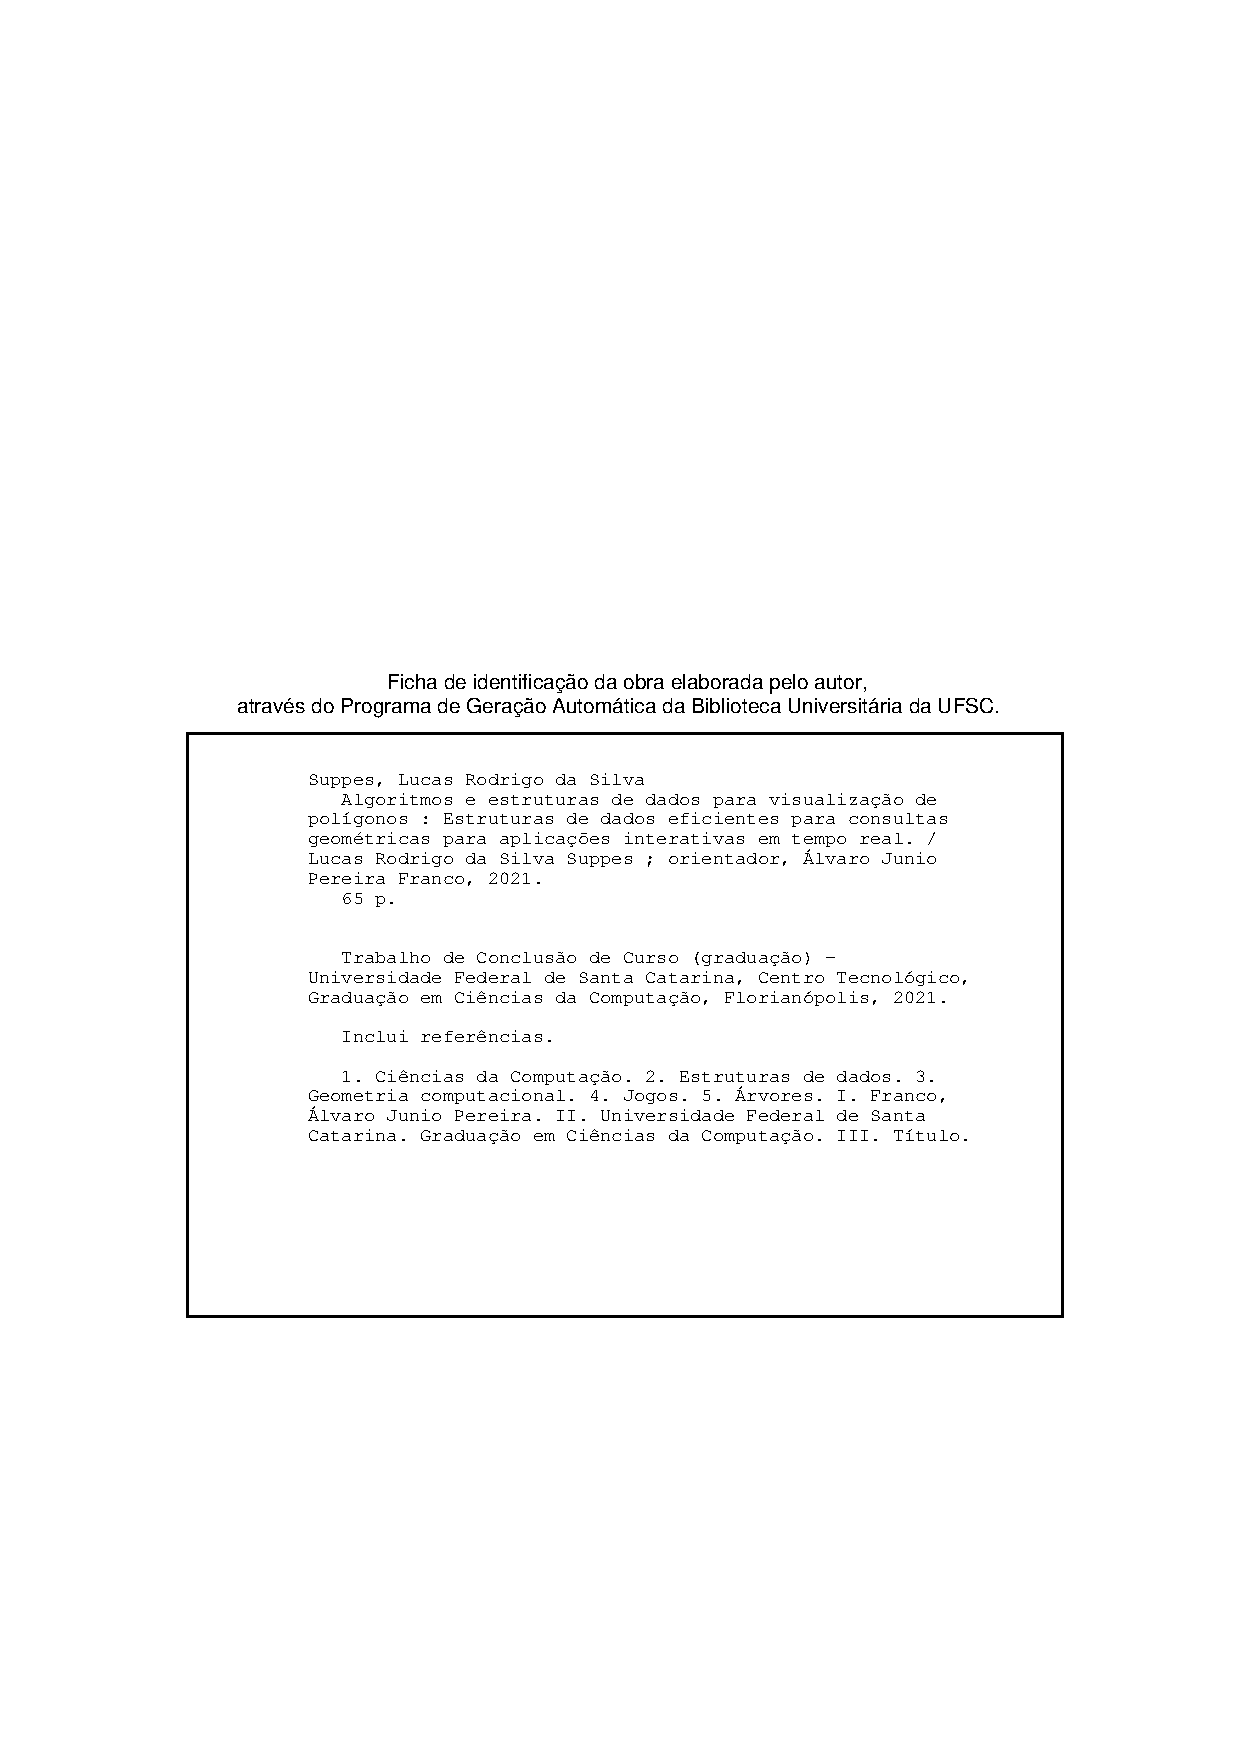
\includepdf{beforetext/Ficha_Catalografica.pdf}
\end{fichacatalografica}
% ---

% ---
% Inserir folha de aprovação
% ---

% Isto é um exemplo de Folha de aprovação, elemento obrigatório da NBR
% 14724/2011 (seção 4.2.1.3). Você pode utilizar este modelo até a aprovação
% do trabalho. Após isso, substitua todo o conteúdo deste arquivo por uma
% imagem da página assinada pela banca com o comando abaixo:
%
% \includepdf{folhadeaprovacao_final.pdf}
%
\begin{folhadeaprovacao}

  \begin{center}
    {\ABNTEXchapterfont\large\imprimirautor}

    \vspace*{\fill}\vspace*{\fill}
    \begin{center}
      \ABNTEXchapterfont\bfseries\Large\imprimirtitulo
    \end{center}
    \vspace*{\fill}
    
    \hspace{.45\textwidth}
    \begin{minipage}{.5\textwidth}
        \imprimirpreambulo
    \end{minipage}%
    \vspace*{\fill}
   \end{center}
        
   %Trabalho aprovado. \imprimirlocal, 22 de abril de 2021:
   Trabalho submetido à banca. Florianópolis, 16 de abril de 2021:

   \assinatura{\textbf{\imprimirorientador} \\ Orientador} 

   %\assinatura{\textbf{Professor} \\ Convidado 3}
   %\assinatura{\textbf{Professor} \\ Convidado 4}
      
   \begin{center}
    \vspace*{0.5cm}
    {\large\imprimirlocal}
    \par
    {\large\imprimirdata}
    \vspace*{1cm}
  \end{center}
  
\end{folhadeaprovacao}
% ---

% ---
% Dedicatória
% ---
\begin{dedicatoria}
   \vspace*{\fill}
   \centering
   \noindent
   \textit{ Este trabalho é dedicado às crianças adultas que,\\
   quando pequenas, sonharam em se tornar cientistas.} \vspace*{\fill}
\end{dedicatoria}
% ---


\begin{agradecimentos}
% Os agradecimentos principais são direcionados à Gerald Weber, Miguel Frasson,
% Leslie H. Watter, Bruno Parente Lima, Flávio de Vasconcellos Corrêa, Otavio Real
% Salvador, Renato Machnievscz\footnote{Os nomes dos integrantes do primeiro
% projeto abn\TeX\ foram extraídos de
% \url{http://codigolivre.org.br/projects/abntex/}} e todos aqueles que
% contribuíram para que a produção de trabalhos acadêmicos conforme
% as normas ABNT com \LaTeX\ fosse possível.

% Agradecimentos especiais são direcionados ao Centro de Pesquisa em Arquitetura
% da Informação\footnote{\url{http://www.cpai.unb.br/}} da Universidade de
% Brasília (CPAI), ao grupo de usuários
% \emph{latex-br}\footnote{\url{http://groups.google.com/group/latex-br}} e aos
% novos voluntários do grupo
% \emph{\abnTeX}\footnote{\url{http://groups.google.com/group/abntex2} e
% \url{http://abntex2.googlecode.com/}}~que contribuíram e que ainda
% contribuirão para a evolução do \abnTeX.
À minha mãe Cleonice que em nenhum momento teve duvidas de minha capacidade e sempre incentivou que eu trilhasse meu rumo qualquer que fosse a direção. Sempre confiou na minha bússola e compasso moral que me guiaram até onde me encontro.

À meu pai Bernardino que sem seu sopro e força jamais teria ido longe. \textit{`` Vós sois os arcos dos quais vossos filhos são arremessados como flechas vivas.'' - Khalil Gibran}

Ao meu orientador Álvaro por esse ano de trabalho incessante e seu grande carinho e suporte para que eu conseguisse executar esta obra.

À cada amigo e colega que conheci durante essa jornada. Dos que ficaram e dos que se foram. Cada letra deste trabalho tem um pouco de cada um.

À cada professor e profissional desta universidade que me passou um pouco de seu conhecimento, e em especial, à aqueles poucos professores que conseguiram  de forma especial cativar minha curiosidade para esta sublime ciência.

À flor que sem ela este trabalho jamais teria vindo a fruição. Por sempre ter acreditado em mim mesmo quando nem eu mesmo acreditava; por cada sorriso mesmo quando eu era só lagrimas; por ter sido meu alicerce quando eu era fraco.

À Ele que dá-me forças, guia-me, protege-me e orienta-me sempre.

\end{agradecimentos}


% ---
% Epígrafe
% ---
\begin{epigrafe}
    \vspace*{\fill}
    \begin{flushright}
		\textit{``Um processo computacional é de fato muito parecido como a ideia de um espirito para os magos. Não pode ser visto ou tocado. Não é composto de matéria. Entretanto, é real. Pode realizar trabalho intelectual. Pode responder questões. Pode afetar o mundo entregando dinheiro em um caixa de banco ou controlando um braço robótico em uma fábrica. Nós conjuramos programas como os magos conjuram suas magias. Eles são cuidadosamente compostos de expressões simbólicas em linguagens de programação arcanas e esotéricas que descrevem o intento para os processos executarem .'' \\
		(Structure and Interpretation of Computer Programs, pagina 2)}
	\end{flushright}
	\begin{flushright}
		\textit{``Ainda que eu andasse pelo vale da sombra da morte, \\
		não temeria mal algum, porque tu estás comigo;\\
		a tua vara e o teu cajado me consolam.\\
		(Bíblia Sagrada, Salmos 23:4)}
	\end{flushright}
\end{epigrafe}
% ---

%
% ---
% RESUMOS
% ---

% resumo em português
\setlength{\absparsep}{18pt} % ajusta o espaçamento dos parágrafos do resumo
\begin{resumo}
	\SingleSpacing
	Este trabalho apresenta um estudo de algumas estruturas de dados e técnicas para processamento de janelas. Estudamos maneiras de estruturar objetos geométricos de tal forma que consultas em janelas são respondidas eficientemente. As estruturas de dados que estudamos foram Árvore $KD$, Árvore de Alcance, Árvore de Intervalos e Árvore de Segmentos. Este trabalho utilizou todas as estruturas de dados no plano. As estruturas de dados e algoritmos de construção e consulta foram implementados. Por fim, utilizamos nossas implementações em uma aplicação que processa pontos e segmentos no plano. 
	%Tendo em mente o constante crescimento de polígonos dos objetos a serem processados, há uma necessidade de que os objetos sejam acessados de forma rápida e eficiente.

	\textbf{Palavras-chave}: Estruturas de Dados. Árvores. Geometria Computacional.
\end{resumo}

% resumo em inglês
\begin{resumo}[Abstract]
	\SingleSpacing
	\begin{otherlanguage*}{english}
		This work presents a study of some data structures and techniques to process windows. We study ways to structure geometric objects in such a way that queries in windows are quickly answered. The data structures that we study were $KD$ Tree, Range Tree, Interval Tree and Segment Tree. This work used all the data structures on the plan. The data structures and the algorithms of construction and query were implemented. Finally, we used our implementation in an application that processes points and segments on the plan.  %A study of the most common tecniques for optimizing rendering on windows.
		%Beign awere of the constant growth of the polygon count and the size of graphical applications, and the necessity for easy and quick access to the objects.

		\textbf{Keywords}: Data Structures. Trees. Computational Geometry.
	\end{otherlanguage*}
\end{resumo}



% ---
% inserir lista de ilustrações
% ---
\pdfbookmark[0]{\listfigurename}{lof}
\listoffigures*
\cleardoublepage
% ---

% ---
% inserir lista de tabelas
% ---
\pdfbookmark[0]{\listtablename}{lot}
\listoftables*
\cleardoublepage
% ---

% ---
% inserir lista de abreviaturas e siglas
% ---
%\begin{siglas}
%  \item[ABNT] Associação Brasileira de Normas Técnicas
%  \item[abnTeX] ABsurdas Normas para TeX
%\end{siglas}
% ---

% ---
% inserir lista de símbolos
% ---
%\begin{simbolos}
%  \item[$ \Gamma $] Letra grega Gama
%  \item[$ \Lambda $] Lambda
%  \item[$ \zeta $] Letra grega minúscula zeta
%  \item[$ \in $] Pertence
%\end{simbolos}
% ---

% ---
% inserir o sumario
% ---
\pdfbookmark[0]{\contentsname}{toc}
\tableofcontents*
\cleardoublepage
% ---

